\chapter{Introduction}
\label{ch:Introduction}
%%% Presentar el tema: Aerial co-workers: a task planning approach for multi-drone teams supporting inspection operations
% Definir el problema
\lettrine[lraise=-0.1, lines=2, loversize=0.2]{T}{he} use of \glspl{UAV} has grown considerably in recent years for numerous applications including real-time monitoring, search and rescue, providing wireless coverage, security and surveillance, precision agriculture, package delivery and infrastructure inspection \cite{CivilAplications}. With the rapidly developing technology in this area, and demonstrations of what \glspl{UAV} can do, there are increasing efforts to bring this technology to other applications. With the expected increase in applications for this technology, new problems and challenges arise, including autonomy, safety, obstacle avoidance and coordination of multi-\gls{UAV} teams. Developing the technology to solve these problems will be a major effort, but as \glspl{UAV} have proven to be critical in situations where humans are at high risk or highly inefficient, and they have proven their capacity to evolve and develop even more potential in the short term, companies are investing in developing all sort of \gls{UAV}-based solutions.

\section{Motivation}
\label{sec:Motivation}
%%% Capi: motivación del problema:
With the increase in global electricity demand, a challenge has arisen for electricity supply companies to maintain and repair power grids in a way that minimizes the frequency of outages. According to \cite{PowerOutagesCauses}, one of the main causes of power outages is damage to transmission lines due to bad weather or inefficient inspection campaigns.

\begin{figure}[htbp]
    \centering
    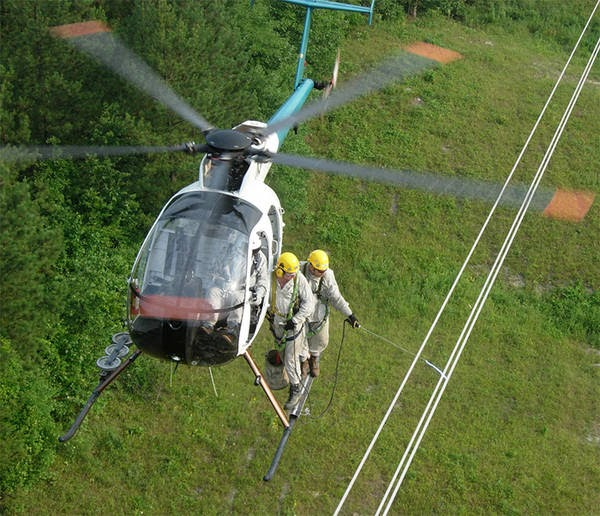
\includegraphics[width=0.6\linewidth]
    {Introduction/figures/helicopter.jpg}
    \caption{Operators getting off the helicopter during a maintenance mission}
    \label{fig:helicopter}
\end{figure}

The strategy often used by electric companies to reduce power outages is to schedule periodic maintenance operations on active lines. This is the most suitable method if the correct functioning of the system is to be ensured and when replacing a circuit is unacceptable \cite{PowerOutagesCauses}. These maintenance missions are carried out by experienced crews on board helicopters and equipped with safety suits and harnesses among other things that prevent the operators from receiving an electric shock (see figure \ref{fig:helicopter}). The problem with this solution is that these activities are dangerous for the operators, as they are working at high altitude and on electrified lines, are extremely time-consuming and expensive (\$1500 per hour) and are subject to human error \cite{MaintenanceCost}.

% Por qué interesan los equipos multi-UAV para la inspección, principales barreras, etc. Puedes hablar del proyecto AERIAL-CORE como contexto del trabajo. Coje texto del paper que te pasé y del proyecto de tesis.
These are the reasons why distribution companies have the need to develop more efficient and safer maintenance methods. Multiple solutions have been proposed to automate this task \cite{MaintenanceSolutions}, but the best of them seems to be the use of \glspl{UAV} because of their flexibility and ability to inspect at different levels \cite{PowerOutagesCauses}. To achieve this, there are still some important barriers to overcome, such as the limited autonomy of these devices, the strong electromagnetic interference to which they would be subjected due to being close to power lines and the ability to detect and avoid obstacles of different nature that can be found in this type of environment \cite{MaintenanceCost}. Providing \glspl{UAV} with the cognitive capability to operate autonomously in such dynamic environments and with the presence of humans, and providing them with a rapid on-line planning method \cite{FastOnlinePlanning}, is key to address these complexities and to safely and successfully accomplish the assigned mission with \gls{UAV} fleets.

%%% Contexto y justificación del trabajo: 
% Dar razones de por qué es útil diseñar un planificador de tareas para equipos multi-UAV
A versatile and reliable software architecture will be essential to integrate and interconnect all the heterogeneous components that compose these cognitive multi-\gls{UAV} systems. In \cite{AerialCoreMulti-Layer}, as part of the AERIAL-CORE European project\footnote{AERIAL-CORE European project homepage: \url{https://aerial-core.eu/}}, a multi-layer software architecture is presented for carrying out such missions cooperatively between human operators and a fleet of quadrotors. One of the layers of software that compose it is a high-level task planner. Its function is to coordinate the entire fleet of \glspl{UAV} to generate high-level behaviours in order to efficiently, safely and successfully complete the maintenance or inspection mission. This type of work has the characteristic of being dynamic, since it is not possible to know in advance what the outcome of the inspection as such will be in order to plan offline, but rather, as the mission develops, new tasks will arise that the fleet will have to attend to. Therefore, the task planner should be able to react to unexpected events (new task, failure of a \gls{UAV}, loss of connection, less autonomy than calculated, etc.) and to replan online. Thus, this layer will be the main cognitive block of the system \cite{AerialCoreMulti-Layer}.

\section{Objectives}
\label{sec:Objectives}
%%%: objetivos que se quieren alcanzar en tu TFM en concreto, dentro de todo el problema.
% Hablar en general del proyecto y de lo que quiero hacer.
The overall objective of this project was to develop a cognitive task planner that would be in charge of governing the behaviour of multi-\gls{UAV} teams for the inspection and maintenance of power lines in a collaborative way with human operators, being one of the software layers that compose the aforementioned software architecture \cite{AerialCoreMulti-Layer} developed for the AERIAL-CORE European project. The fleet of governed \glspl{UAV} acts as an aerial co-worker and can perform various tasks such as delivering a tool to an operator, inspecting regions of the power line or monitoring a worker while operating to ensure his safety. The planner receives both high-level input and feedback from the different equipments that make up the fleet, and processes all the information to elaborate a plan to manage the \gls{UAV} team or modify it in reaction to an unforeseen event. To achieve this, the following objectives were defined:

\begin{itemize}
    \item Ensure that resources are used and tasks are executed efficiently.
    \item Comply with all security requirements and ensure the integrity of equipment and mission success.
    \item Be able to replan online to react to unforeseen events.
    \item Implement the software layer in \gls{ROS} and manage the necessary communications with the rest of the software layers and modules that make up the architecture.
    \item Carry out \gls{SITL} simulations to prove that the algorithm is able to govern the behaviour of the fleet efficiently and safely, and that it is able to react to unforeseen events dynamically, demonstrating cognitive capabilities.
\end{itemize}

%%% Preguntas de investigación e hipótesis: 
% Enumerar las hipótesis realizadas para diseñar el planificador

%\begin{hypothesis}\label{hyp:inicial}
%    "".
%\end{hypothesis}

\endinput